\documentclass{article}
\usepackage{amsmath}
\usepackage{amssymb}
\usepackage{amsbsy}
\usepackage{bbm}
\usepackage{url}
\usepackage{color}
\usepackage{graphicx}
\usepackage{epstopdf}
\usepackage{fancyhdr}
\usepackage{enumerate}
\usepackage{tikz}
\usepackage[ruled,vlined]{algorithm2e}
\usepackage[colorlinks=true,urlcolor=blue]{hyperref}
\usepackage[utf8]{inputenc}
\usepackage{float}

\title{Homework 3}
\author{John Doe, jdoe@stanford.edu}

\newcommand{\Solution}[1]{{\medskip \color{black} \bf $\bigstar$~\sf \textbf{Solution}~$\bigstar$ \sf #1 } \bigskip}

\begin{document}

\maketitle

\section{GraphRNN [20 points]}

In class, we covered GraphRNN, a generative model for graph structures. Here we assume that the graph has no node types/features, and no edge types/features.

\subsection{Edge-level RNN [12 points]}
Remember that GraphRNN uses random BFS ordering to generate graphs by
iteratively adding a node and predicting its connectivity to the nodes already in the graph. Suppose that the GraphRNN model is generating a grid graph:
\begin{figure}[H]
    \centering
    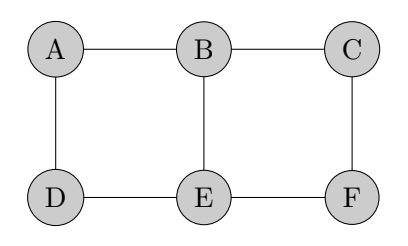
\includegraphics[width=0.4\textwidth]{hw3-q1.jpg}
    \caption{GraphRNN grid graph.}
\end{figure}
If we wanted a GraphRNN to generate this graph, what predictions would each cell in the edge-level RNN need to make? Recall that a GraphRNN needs to predict, for each new node, which existing nodes it needs to wire an edge with. It outputs 1 when there should be an edge, and 0 when there should not. Nodes are added in BFS ordering starting from Node A. Assume that when exploring the neighbors of a node, they are explored in alphabetical order.\\

\Solution{Write your answer here. \\ Example for writing a matrix $M$: \\
 \[M = 
    \begin{bmatrix}
    1 \ 2   \\
    3 \ 4
    \end{bmatrix}
\]
Example for writing an equation:
\begin{equation}
    F=ma
\end{equation}
Example for inserting a figure: 
\begin{figure}[!htb]
\centering
  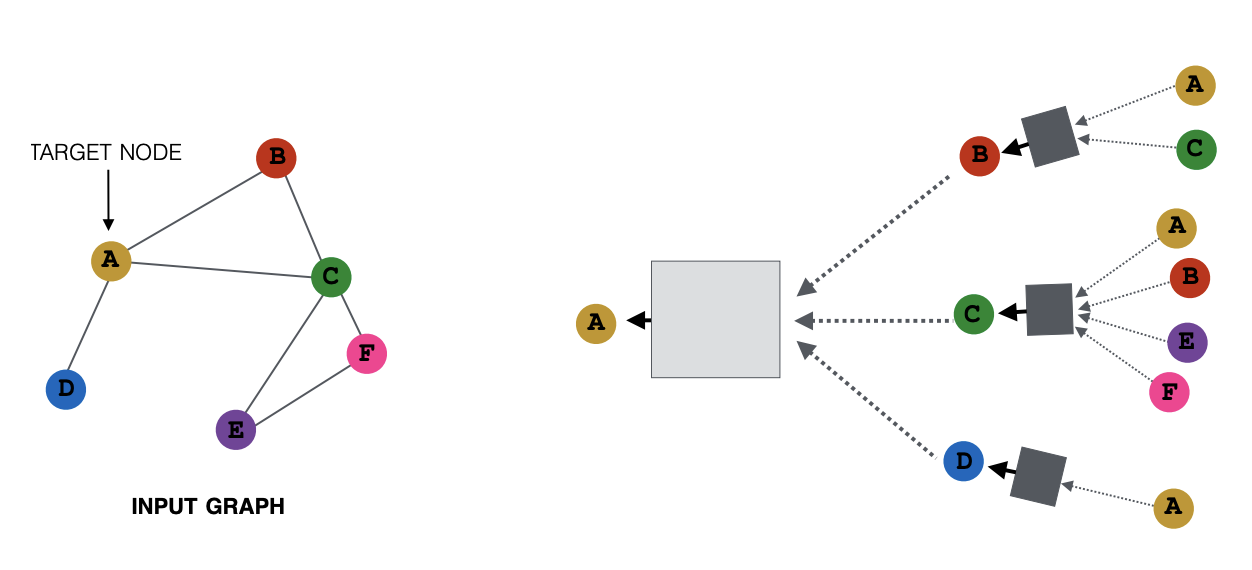
\includegraphics[width=0.8\columnwidth]{Sample_Image.png}
  \label{fig:Q1.1}
\end{figure}
}

\subsection{Advantages of BFS ordering [8 points]}
Explain 2 advantages of graph generation with random BFS ordering of nodes in
the graph, as opposed to generating with a random ordering of nodes in the graph.\\

\Solution{}




\section{Subgraph and Order Embeddings [35 points]}

In lecture, we demonstrated that subgraph matching can be effectively learned by embedding subgraphs into the order embedding space. The reason is that many properties associated with subgraphs are naturally reflected in the order embedding space.

For this question, we say “graph $A$ is a subgraph of graph $B$” when there exists a subgraph of $B$ that is graph-isomorphic to graph $A$. We additionally only consider the induced subgraph setting introduced in lecture, and all the order embeddings are non-negative.

Recall that the order embedding constraint states that: $A$ is a subgraph of $B$ if and only if $z_A[i] \leq z_B[i]$ for all embedding dimension $i$. For simplicity, we do not consider anchor nodes in this question, and assume that the order embedding $z_A$ is an embedding of graph $A$.

\subsection{Transitivity [8 points]}
Show that the subgraph relation is transitive: if graph $A$ is a subgraph of graph $B$, and graph $B$ is a subgraph of $C$, then graph $A$ is a subgraph of $C$. The proof should make use of the subgraph isomorphism definition: if graph $A$ is a subgraph of graph $B$, then there exists a bijective mapping $f$ that maps all nodes in $V_A$ to a subset of nodes in $V_B$, such that the subgraph of $B$ induced by $\{(v)|v \in V_A\}$ is graph-isomorphic to $A$.

\Solution{}

\subsection{Anti-symmetry [8 points]}
Use the same definition on subgraph isomorphism to show that the subgraph relation is anti-symmetric: if graph $A$ is a subgraph of graph $B$, and graph $B$ is a subgraph of graph $A$, then $A$ and $B$ are graph-isomorphic.

Hint: What do these conditions imply about the number of nodes in $A$ and $B$? How does this relate to graph isomorphism?

\Solution{}

\subsection{Common Subgraphs [4 points]}
Consider a 2-dimensional order embedding space. Graph $A$ is embedded into $z_A$, and graph $B$ is embedded into $z_B$. Suppose that the order embedding constraint is perfectly preserved in this order embedding space. Prove that graph $X$ is a common subgraph of $A$ and $B$ if and only if $z_X \preccurlyeq \min\{z_A, z_B\}$. Here $\min$ denotes the element-wise minimum between two embedding vectors.

\Solution{}

\subsection{Order Embedding Constraints [5 points]}
Suppose that graphs $A,B,C$ are non-isomorphic graphs that are not subgraphs of each other. We embed them into a 2-dimensional order embedding space. Without loss of generality, suppose that we compare the values of their embeddings in the first dimension (dimension 0) and have $z_A[0] > z_B[0] > z_C[0]$. What does this imply about the relation among $zA[1],zB[1],zC[1]$, assuming that the order embedding constraint is perfectly satisfied?

\Solution{}

\subsection{Subgraph Relations [10 points]}
In this question, we show that a 2-dimensional order embedding space is not sufficient to perfectly model subgraph relations.

Suppose that graphs $A, B, C$ are non-isomorphic graphs that are not subgraphs of each other. Without loss of generality, suppose $z_A[0] > z_B[0] > z_C[0]$. Can you construct an example of graphs $X,Y,Z$ that are common subgraphs of one or more graphs in $\{A,B,C\}$ (as an example, we can have $X$ be a common subgraph of $A$ and $B$), such that the corresponding embeddings are guaranteed to satisfy $z_X \preccurlyeq z_Y$ and $z_X \preccurlyeq z_Z$? You do not need to specify the embedding coordinates. Just give the subgraph relations among $X, Y, Z$ and $A, B, C$. Please show why your example satisfies the condition.

\textit{Note that this condition implies that $X$ is a common subgraph of $Y$ and $Z$. However, one can construct actual example graphs of $A, B, C, X, Y, Z$ such that $X$ is not a common subgraph of $Y$ and $Z$. This means that 2-dimensional order embedding space cannot perfectly model subgraph relations. Hence in practice we use high-dimensional order embedding space. For this question, you do not have to show such example graphs.}

\Solution{}




\section{Honor Code}
(X) I have read and understood Stanford Honor Code before I submitted my work.
\\ $**$ Collaboration: Write down the names \& SUNetIDs of students you collaborated with on Homework 2 (None if you didn’t).$**$
\\ $**$Note: Read our website on our policy about collaboration!$**$


\end{document}
